\documentclass[tikz,border=2pt]{standalone}
\usepackage{amsmath,amssymb}
\usepackage{tikz}

\begin{document}
% One machine, jobs with processing times (5,20,15), due dates (24,22,35), penalty rates
% (12,19,34). Sequence 2,1,3: completions 20, 25, 40; tardiness 0, 1, 5; penalty 189.
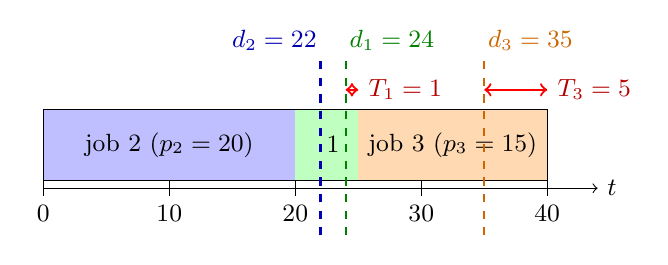
\begin{tikzpicture}[every node/.style={font=\small}, x=0.16cm]
	\fill[blue!25] (0,0) rectangle (20,0.9); \node[font=\small] at (10,0.45) {job 2 ($p_2=20$)};
	\fill[green!25] (20,0) rectangle (25,0.9); \node[font=\small] at (23,0.45) {1};
	\fill[orange!30] (25,0) rectangle (40,0.9); \node[font=\small] at (32.5,0.45) {job 3 ($p_3=15$)};
	\draw (0,0) rectangle (40,0.9);
	\draw[->] (0,-0.1) -- (44,-0.1) node[right, font=\small] {$t$};
	\foreach \t in {0,10,20,30,40} {\draw (\t,-0.0) -- (\t,-0.2) node[below, font=\small] {$\t$};}
	\draw[blue!70!black, dashed, thick] (22,-0.7) -- (22,1.6) node[above left, inner sep=1pt, font=\small] {$d_2=22$};
	\draw[green!50!black, dashed, thick] (24,-0.7) -- (24,1.6) node[above right, inner sep=1pt, font=\small] {$d_1=24$};
	\draw[orange!80!black, dashed, thick] (35,-0.7) -- (35,1.6) node[above right, inner sep=1pt, font=\small] {$d_3=35$};
	\draw[<->, red, thick] (24,1.15) -- (25,1.15) node[right, font=\small, red!70!black] {$T_1=1$};
	\draw[<->, red, thick] (35,1.15) -- (40,1.15) node[right, font=\small, red!70!black] {$T_3=5$};
	\end{tikzpicture}
\end{document}
